\RequirePackage{etex} % needed for worldflags -> else import collision
\documentclass{standalone}
%\standaloneconfig{border=2mm 2mm 2mm 2mm}

\usepackage{tikz}
\usepackage{worldflags}

\def\flipsize{5} % for 5cmx5cm flips
\def\flipwidth{0.1} % width of the flip, here 1.5mm
\def\flipdiameter{3.25} % size of window of the flip
% choose flip diameter as next biggest for coin diamter + coin height

\def\staplelength{0.9} % length of your staples; not currently used

% All text values for the coin go here...
\def\coindenomination{1/2 Dollar}
\def\coindatemint{1964 D}
\def\coincountry{US}
\def\coincatalogreference{KM\#202}
\def\coingrade{AU}

\begin{document}
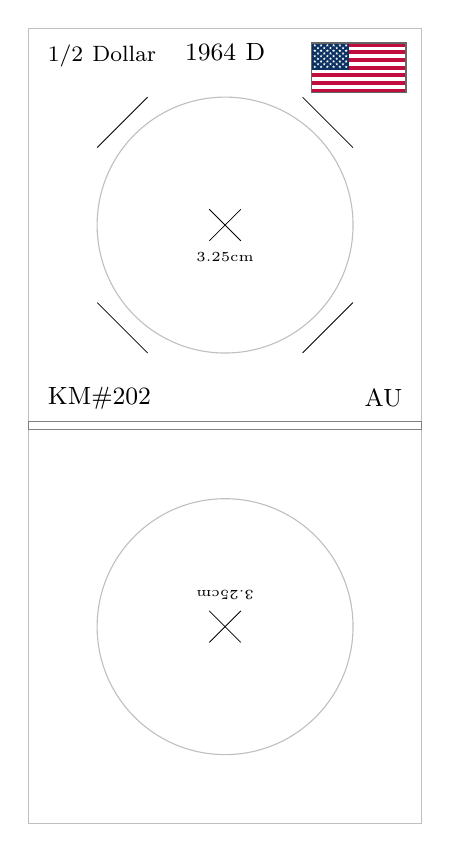
\begin{tikzpicture}
% frame of the whole flip
\draw[draw=lightgray] (0,\flipsize) rectangle (\flipsize,-\flipsize-\flipwidth);
% box for where to fold
\draw[draw=gray] (0,0) rectangle (\flipsize,-\flipwidth);

% grid front and back; for easier debugging
%\draw[lightgray] (0,0) grid (\flipsize,\flipsize);
%\draw[lightgray] (0,0-\flipwidth) grid (\flipsize,-\flipsize-\flipwidth);


% Circle for coin - front side
\coordinate (A) at (\flipsize*0.5, \flipsize*0.5);
\node (circlefront) [draw=lightgray, circle, minimum size = \flipdiameter cm] at (A) {};
% cross in that circle for better cutting
\draw[line width=0.1mm, black] ($(A)+(0.2,0.2)$) -- ($(A)-(0.2,0.2)$) {};
\draw[line width=0.1mm, black] ($(A)+(0.2,-0.2)$) -- ($(A)-(0.2,-0.2)$) {};
% write diameter inside to easier find right flip and adjust cutter
\node[align=center, rotate=0] at ($(A)-(0,0.4)$) {\tiny\flipdiameter cm}; % mm better, but harder
% do markers for staples 
% todo dont hardcode staples, use parameters...
\draw[line width=0.1mm, black] ($(circlefront.north east)+(0.15,0.15)+(0.32,-0.32)$) -- ($(circlefront.north east)+(0.15,0.15)-(0.32,-0.32)$) {};
\draw[line width=0.1mm, black] ($(circlefront.south east)+(0.15,-0.15)+(0.32,0.32)$) -- ($(circlefront.south east)+(0.15,-0.15)-(0.32,0.32)$) {};
\draw[line width=0.1mm, black] ($(circlefront.south west)-(0.15,0.15)+(0.32,-0.32)$) -- ($(circlefront.south west)-(0.15,0.15)-(0.32,-0.32)$) {};
\draw[line width=0.1mm, black] ($(circlefront.north west)-(0.15,-0.15)+(0.32,0.32)$) -- ($(circlefront.north west)-(0.15,-0.15)-(0.32,0.32)$) {};

% circle for coin - back side
\coordinate (B) at (\flipsize * 0.5, -\flipsize * 0.5 -\flipwidth);
\node (circleback) [draw=lightgray, circle, minimum size = \flipdiameter cm] at (B) {};
% cross in that circle for better cutting
\draw[line width=0.1mm, black] ($(B)+(0.2,0.2)$) -- ($(B)-(0.2,0.2)$) {};
\draw[line width=0.1mm, black] ($(B)+(0.2,-0.2)$) -- ($(B)-(0.2,-0.2)$) {};
% write diameter inside to easier find right flip and adjust cutter
\node[align=center, rotate=180] at ($(B)+(0,0.4)$) {\tiny\flipdiameter cm}; % mm better, but harder

% texts and flags
% text denomination
\node[text width=1.5cm, align=left] at (0.2*\flipsize,0.93*\flipsize) {\footnotesize \coindenomination};
% text date and mintmark
\node[text width=1.5cm, align=center] at (0.5*\flipsize,0.94*\flipsize) {\small \coindatemint};
% flag top righ
\pic (flag) [country=\coincountry, width=0mm, length=12mm] at (4.2,4.5) {worldflag};
% text catalog number
\node[text width=1.5cm, align=left] at (0.2*\flipsize,0.3) {\small \coincatalogreference};
% text grade
\node[text width=1.5cm, align=right] at (0.8*\flipsize,0.3) {\small \coingrade};
\end{tikzpicture}
\end{document}